\documentclass[../the.tex]{subfiles}
\begin{document}
{\fontsize{13}{12} \selectfont

Trong phạm vi nghiên cứu này sẽ sử dụng mô hình YOLOv7, YOLOv8, SSD MobileNet. Mục \ref{sec:dataset} mô tả về tập dữ liệu. Mục \ref{sec:model} giới thiệu về các mô hình được sử dụng và sơ đồ hệ thống ở Mục \ref{sec:sodo}

}
\section{Tập dữ liệu}
\label{sec:dataset}

{\fontsize{13}{12} \selectfont

	Trong phạm vi nghiên cứu, các tập dữ liệu sử dụng sẽ là TrashNet \cite{yang2016classification}, TACO \cite{proença2020taco} và bổ sung tập dữ liệu tự thu thập được ở ĐBSCL.
	Tham khảo việc phân loại rác của Yan \cite{yang2016classification} và quá trình thu thập dữ liệu thực tế nhận thấy các loại rác bằng thủy tinh ở môi trường bên ngoài rất thường là các mảnh kính trong suốt nhìn thấy nên hoặc có độ phản chiếu ánh sáng cao nên rất khó phát hiện, vì vậy các thủy tinh sẽ được gom vào các loại rác khác.
	Lớp giấy và thùng giấy sẽ được gom lại vì cùng chất liệu. Cuối cùng mô hình sẽ phân các loại ra làm các lớp:
	\begin{itemize}
		\item Kim loại gồm chủ yếu là các nắp bia, các vỏ bình làm bằng kim loại.
		\item Nhựa - nilon rất phổ biến, gồm các vật liệu làm từ nhựa như ly nhựa, các túi nilon.
		\item Giấy gồm các vật liệu từ giấy, các thùng giấy, vỏ gói thuốc lá, hộp giấy.
		\item Rác khác là các loại rác còn lại với từng loại xuất hiện ít hoặc khó phát hiện như thủy tinh, các vỏ gói đa sắc,
		      mút, vải,\dots
	\end{itemize}
}

\subsection{TrashNet}
\label{sec:trashnet}
{\fontsize{13}{12} \selectfont

	TrashNet là tập dữ liệu được giới thiệu trong bài nghiên cứu của \cite{yang2016classification} bao gồm các lớp và số lượng như Bảng \ref{tab:dataset}. Tất cả hình ảnh được chụp bằng điện thoại Iphone7 sử dụng ánh sáng mặt trời hoặc ánh sáng phòng, các đối tượng được chụp trong nền trắng hoặc bao quát toàn bộ khung hình, một số hình ảnh ở tập Trashnet ở hình
	\ref{fig:dataset_0}.
	Do mục đích ban đầu của tập dữ liệu dùng để phân lớp nên nghiên cứu phải thực hiện gán hộp giới hạn cho bộ dữ liệu để phù hợp với nhu cầu phát hiện đối tượng. Tập dữ liệu TrashNet bao gồm các đối tượng có kích thước lớn và rõ ràng, mục đích sử dụng tăng độ nhận dạng cho mô hình. Bảng \ref{tab:dataset1} thể hiện số lượng đối tượng sau khi đã gán hộp giới hạn cho tập dữ liệu, hình
	\ref{fig:dataset_1} mô tả tập dữ liệu TrashNet khi được gán hộp giới hạn.

}

\begin{table}[!ht]
	\centering
	\caption{Số lượng ảnh theo lớp của tập dữ liệu TrashNet}
	\begin{tabular}{|l|l|r|}
		\hline
		\multicolumn{1}{|l|}{
			\textbf{\#}}
		 & \multicolumn{1}{c|}{\textbf{Lớp}}
		 & \multicolumn{1}{c|}{\textbf{Số lượng ảnh}} \\
		\hline

		1
		 & Cardboard
		 & 403                                        \\
		\hline

		2
		 & Paper
		 & 594                                        \\
		\hline

		3
		 & Glass
		 & 501                                        \\
		\hline

		4
		 & Plastic
		 & 482                                        \\
		\hline

		5
		 & Metal
		 & 410                                        \\
		\hline

		6
		 & Trash
		 & 137                                        \\
		\hline


		\textbf{Tổng cộng}
		 &
		 & 2524                                       \\
		\hline
	\end{tabular}

	\label{tab:dataset}
\end{table}

\begin{figure}[H]
	\centering
	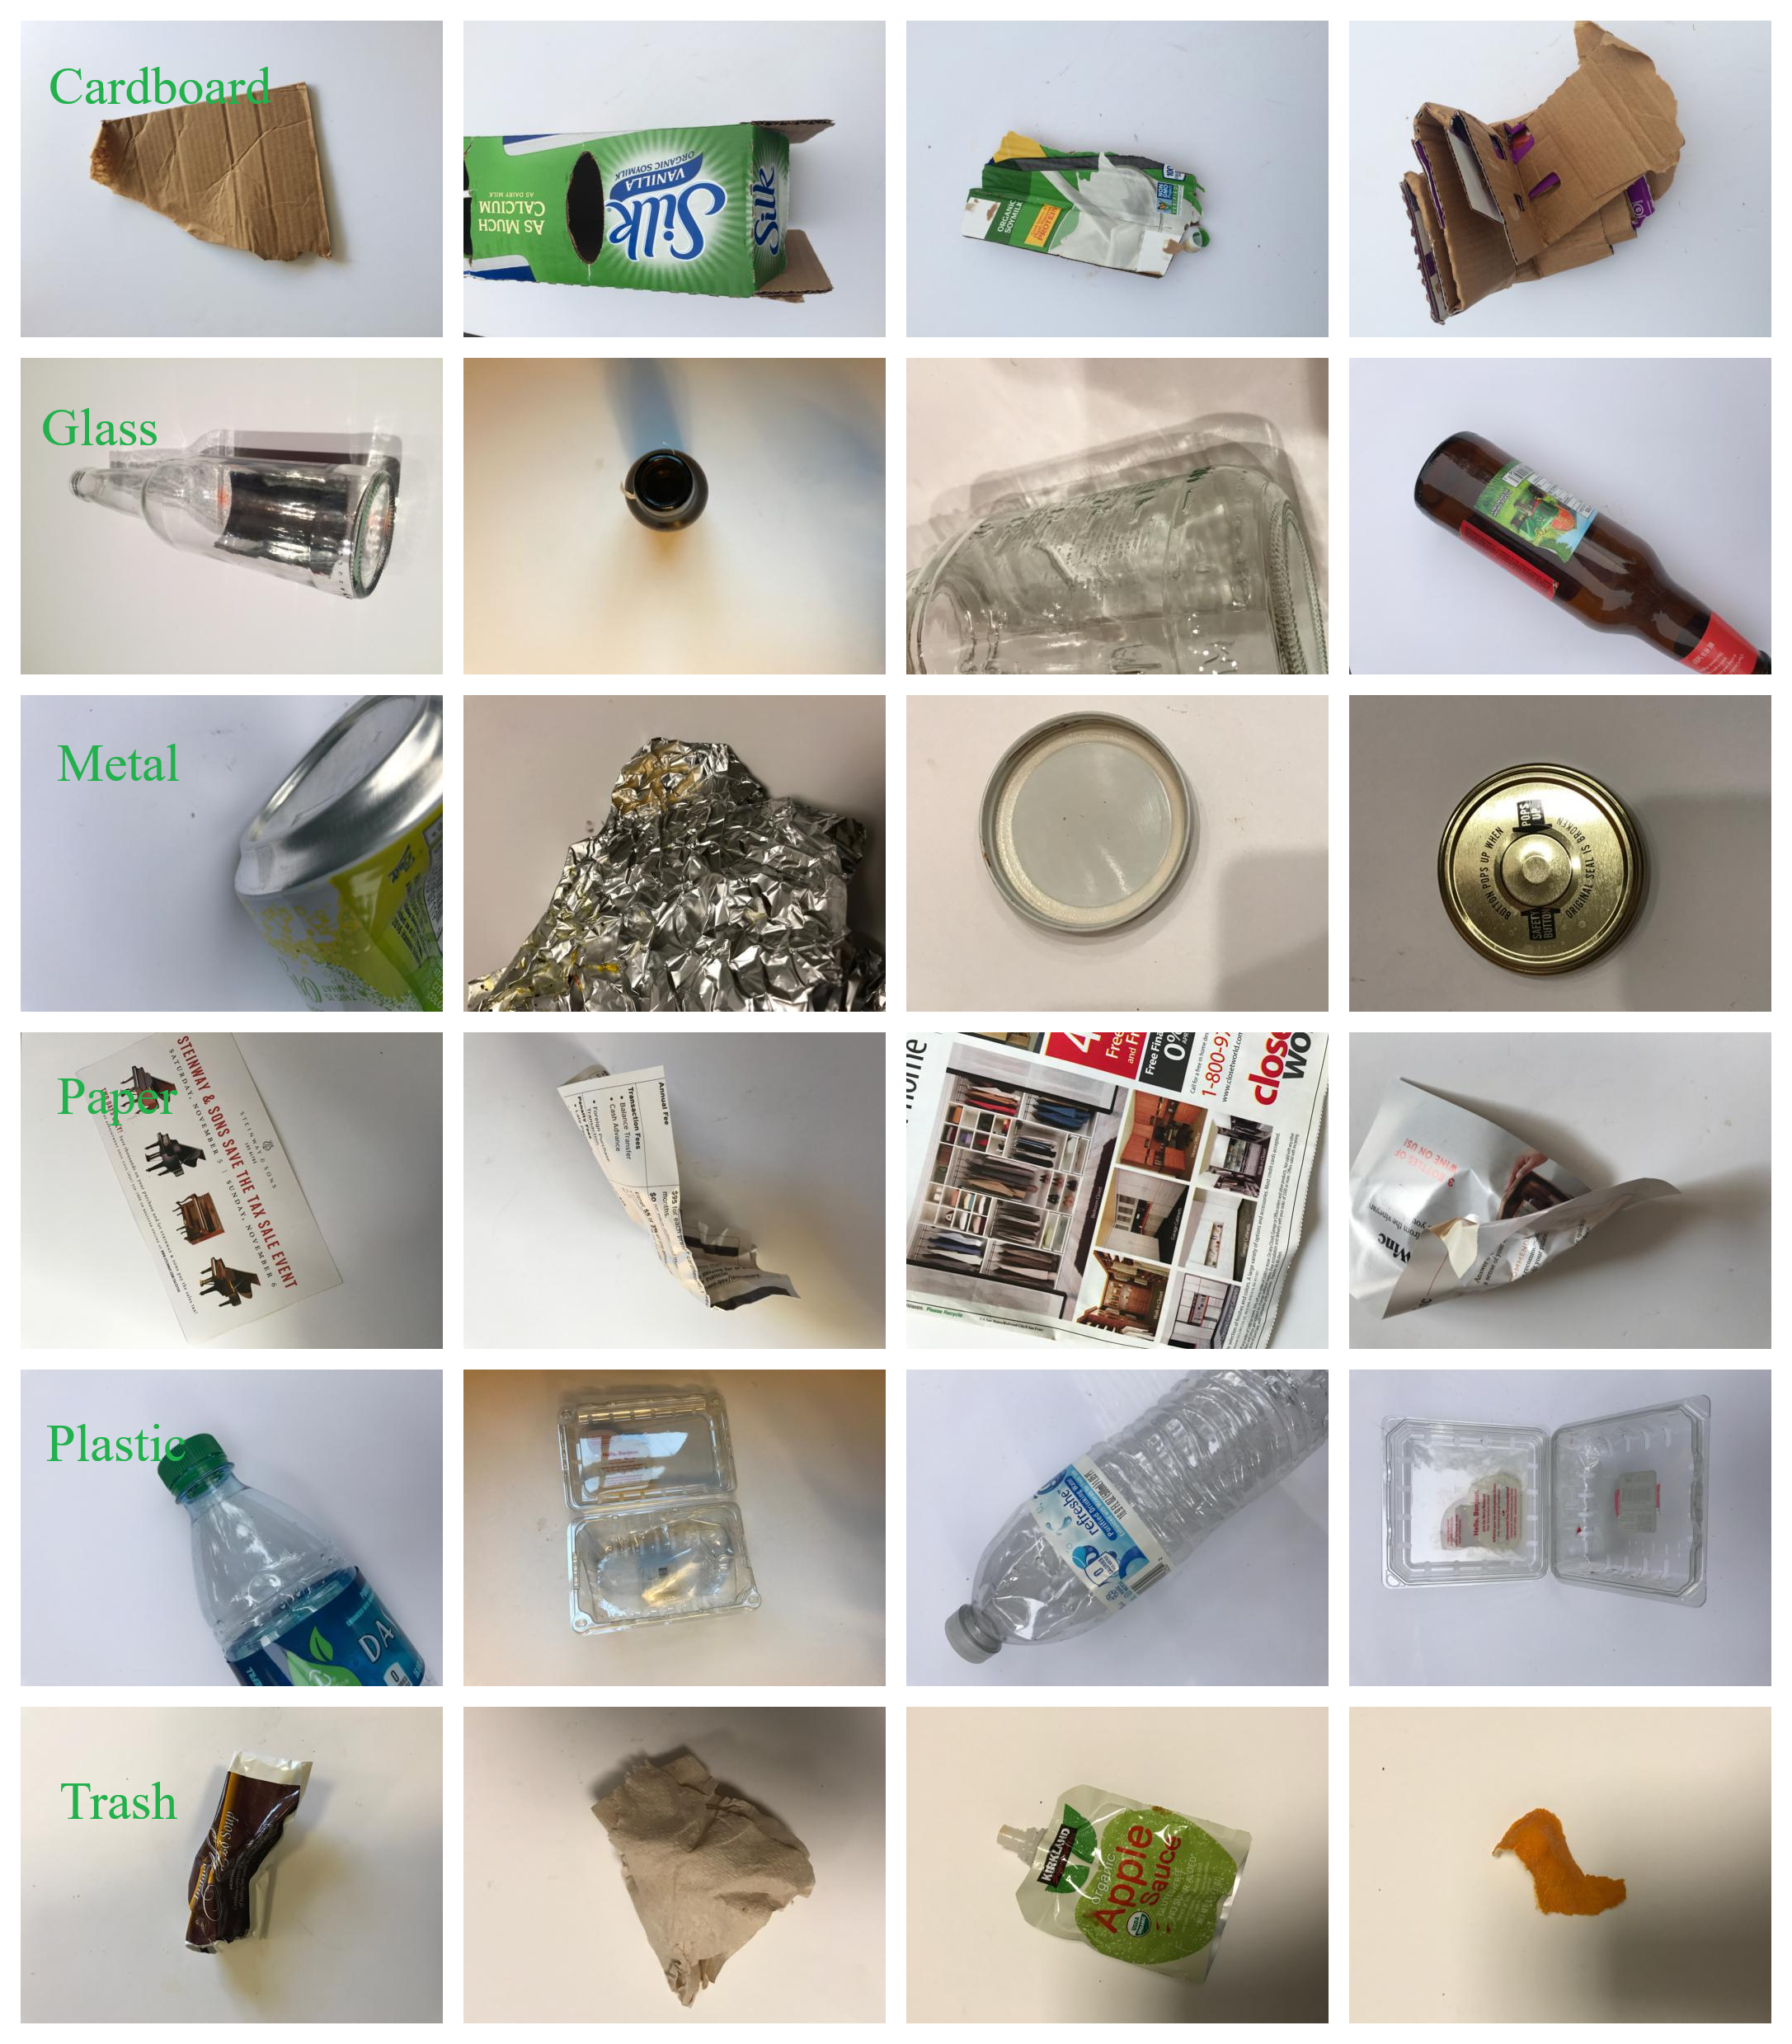
\includegraphics[width=1\textwidth]{trashnet_sample.png}
	\caption{Ví dụ về hình ảnh của tập dữ liệu TrashNet}
	\label{fig:dataset_0}
\end{figure}

\begin{table}[!ht]
	\centering
	\caption{Số lượng ảnh theo lớp của tập dữ liệu TrashNet khi được gán hộp giới hạn}
	\begin{tabular}{|l|l|r|}
		\hline
		\multicolumn{1}{|l|}{
			\textbf{\#}}
		 & \multicolumn{1}{c|}{\textbf{Lớp}}
		 & \multicolumn{1}{c|}{\textbf{Số lượng vật thể}} \\
		\hline

		1
		 & Cardboard
		 & 404                                            \\
		\hline

		2
		 & Paper
		 & 601                                            \\
		\hline

		3
		 & Glass
		 & 509                                            \\
		\hline

		4
		 & Plastic
		 & 479                                            \\
		\hline

		5
		 & Metal
		 & 410                                            \\
		\hline

		6
		 & Trash
		 & 149                                            \\
		\hline


		\textbf{Tổng cộng}
		 &
		 & 2552                                           \\
		\hline
	\end{tabular}

	\label{tab:dataset1}
\end{table}

\begin{figure}[H]
	\centering
	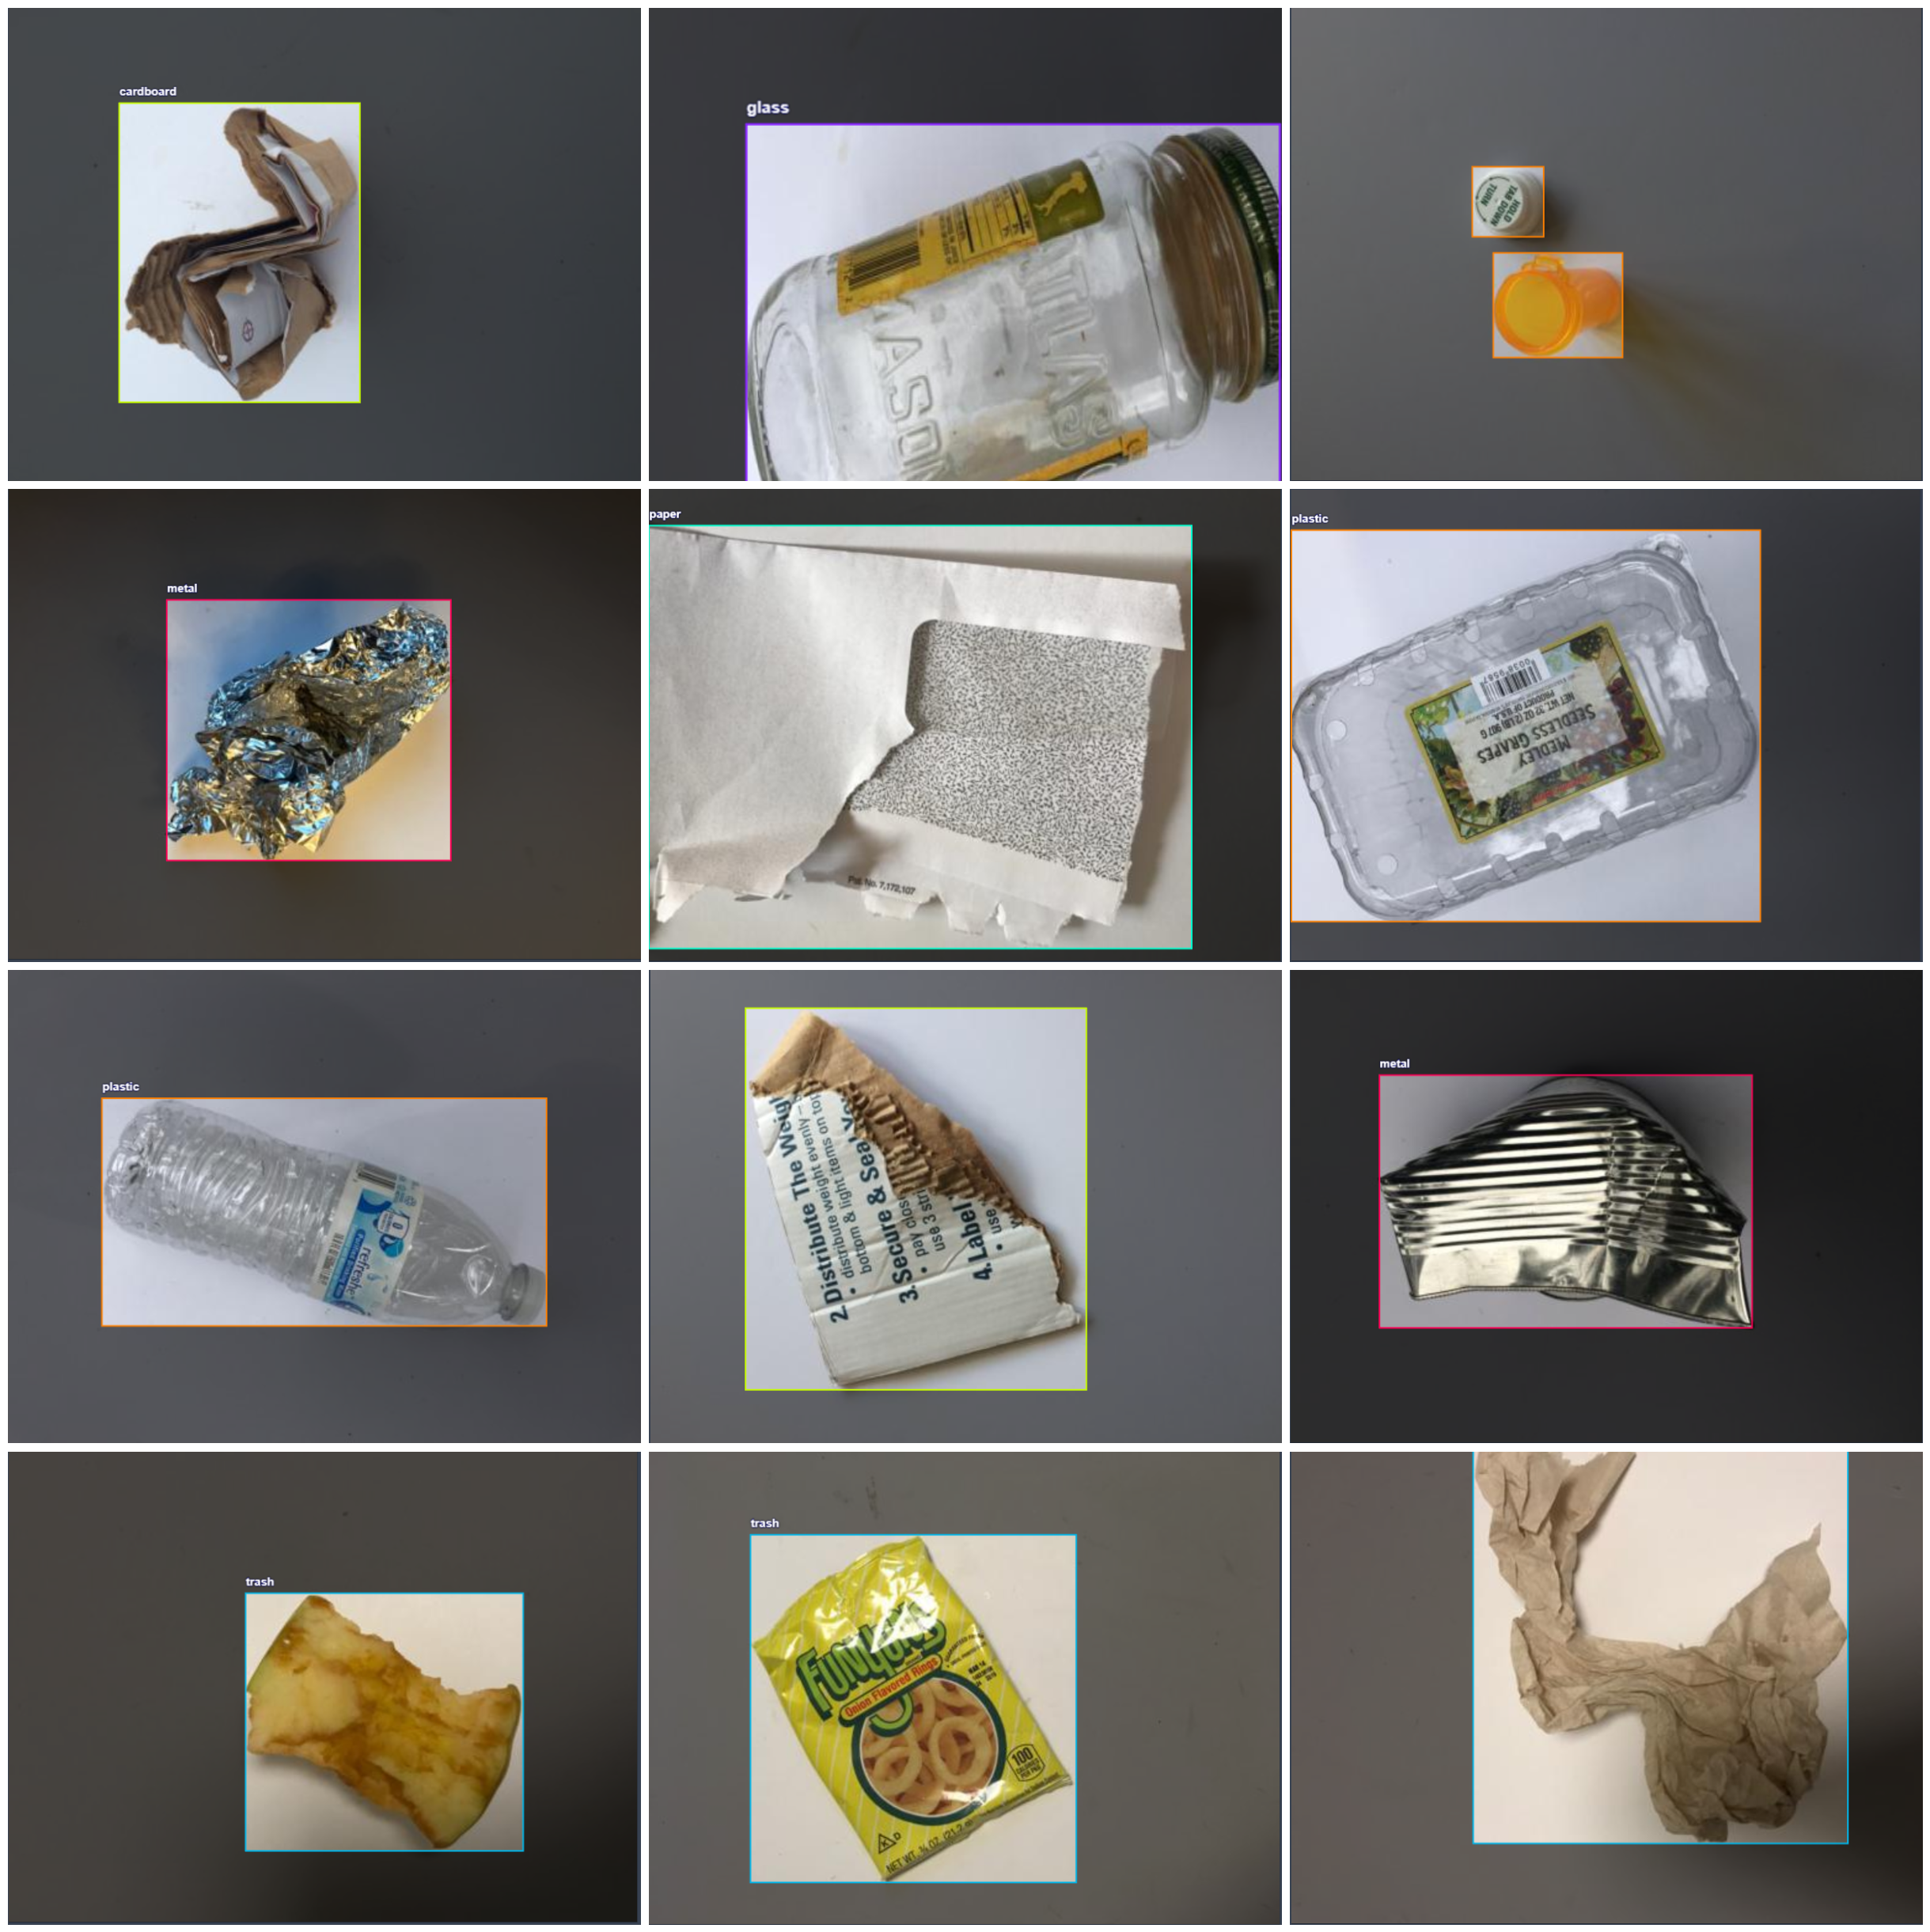
\includegraphics[width=1\textwidth]{trashnet_sample2.png}
	\caption{Ví dụ về hình ảnh của tập dữ liệu TrashNet được gán hộp giới hạn}
	\label{fig:dataset_1}
\end{figure}

\subsection{TACO}
\label{sec:TACO}
{\fontsize{13}{12} \selectfont

	TACO là một tập dữ liệu hình ảnh về chất thải trong tự nhiên. Tập dữ liệu chứa các hình ảnh về rác được chụp trong nhiều môi trường khác nhau, từ những bãi biển đến đường phố London. Những hình ảnh này được gắn nhãn và phân đoạn thủ công để đào tạo và đánh giá các thuật toán phát hiện đối tượng.
	Hiện tại bộ dữ liệu có 1.500 ảnh với 4.784 vật thể
	và 3.918 ảnh mới cần được gán nhãn. Một số hình ảnh của tập dữ liệu ở Hình \ref{fig:dataset_taco}

}

\begin{figure}[H]
	\centering
	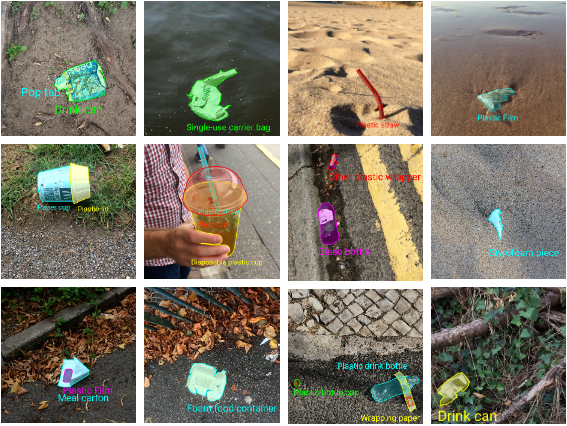
\includegraphics[width=1\textwidth]{Taco.png}
	\caption{Ví dụ về hình ảnh của bộ dữ liệu TACO \cite{proença2020taco}}
	\label{fig:dataset_taco}
\end{figure}


{\fontsize{13}{12} \selectfont
Bộ dữ liệu TACO được cung cấp theo chuẩn json của COCO (xem Hình \ref{fig:coco_full_format}).
Các trường dữ liệu cung cấp thông tin về giấy phép, đường dẫn các hình ảnh, thông tin về danh mục, ngữ cảnh và đặc biệt là thông tin gán nhãn của đối tương được lưu ở trường \textbf{annotations}.
Hình \ref{fig:taco_format} mô tả các chi tiết về một đối tượng được gán nhãn gồm hình ảnh chứa đối tượng, nhãn, diện tích, đa giác phân đoạn và hộp giới hạn. Hộp giới hạn được lưu theo cấu trúc $[x,y,width,height]$ lần lượt là tọa độ điểm, chiều rộng, chiều cao.

}

\begin{figure}[H]
	\centering
	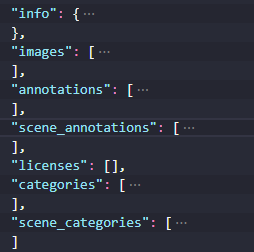
\includegraphics[width=0.5\textwidth]{COCO_format.png}
	\caption{Cấu trúc tệp theo chuẩn COCO của dữ liệu TACO}
	\label{fig:coco_full_format}
\end{figure}

\begin{figure}[H]
	\centering
	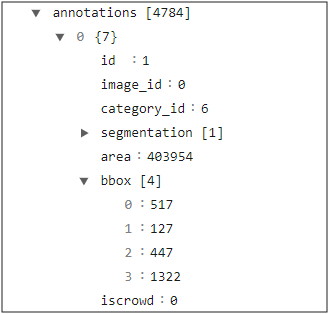
\includegraphics[width=0.5\textwidth]{COCO_full_format.png}
	\caption{Cấu trúc lưu trữ thông tin một đối tượng được gán nhãn trong bộ dữ liệu TACO}
	\label{fig:taco_format}
\end{figure}

{\fontsize{13}{12} \selectfont

Bộ dữ liệu gồm 28 danh mục lớn  (xem Hình \ref{fig:dataset_taco_1_a}) và 60 danh mục nhỏ (xem Hình \ref{fig:dataset_taco_1_b}) với
6 loại nền là rác, thảm cỏ, nước, trong nhà, vỉa hè, cát đá (xem Hình \ref{fig:dataset_taco_1_c}). Bộ dữ liệu TACO thể hiện sự đa dạng trong từng loại rác,
tuy nhiên đó cũng là sự hạn chế khi có những lớp có quá ít dữ liệu như Carded blister pack (1 đối tượng), Battery (2 đối tượng), và các lớp có quá nhiều đối tượng như Cigarette (667 đối tượng) và Unlabeled litter (516 đối tượng).

}

\begin{figure}[H]
	\centering
	\subfloat[\centering {\fontsize{11}{10} \selectfont Danh mục lớn }]{{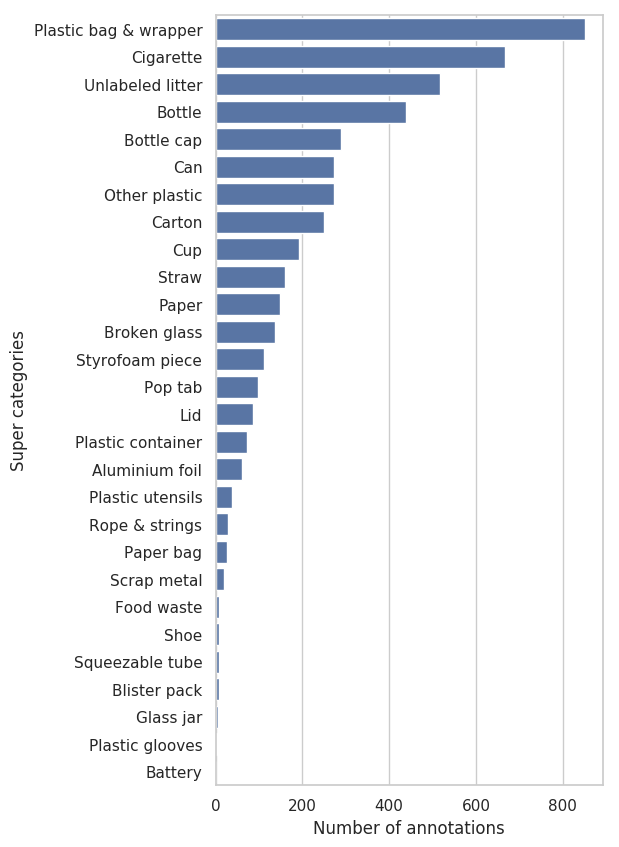
\includegraphics[width=7cm]{taco_super.png} \label{fig:dataset_taco_1_a}}}%
	\qquad
	\subfloat[\centering {\fontsize{11}{10} \selectfont Danh mục nhỏ}]{{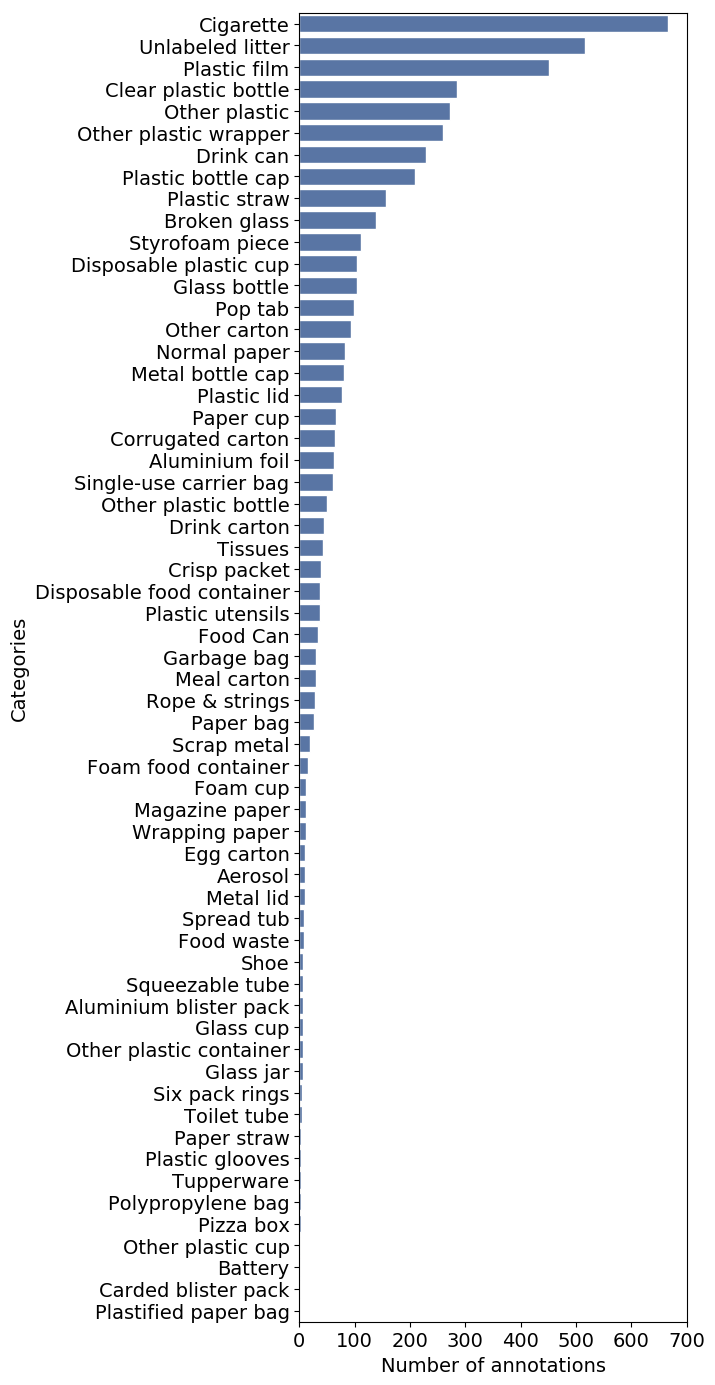
\includegraphics[width=7cm]{taco_cat.png} \label{fig:dataset_taco_1_b}}}%
	\qquad
	\subfloat[\centering {\fontsize{11}{10} \selectfont Tỉ lệ nền}]{{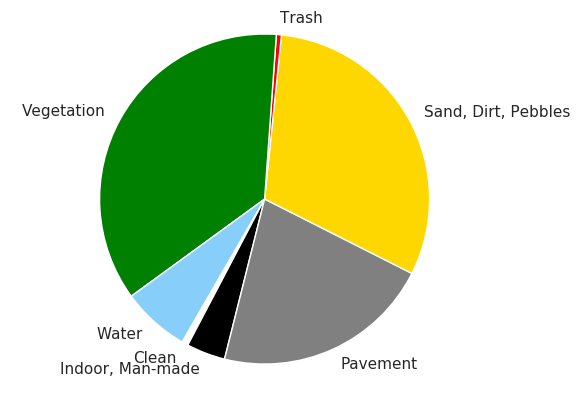
\includegraphics[width=10cm]{taco_bg.png} \label{fig:dataset_taco_1_c}}}%
	\caption{Các thống kê theo danh mục lớn, danh mục nhỏ, tỉ lệ nền của bộ dữ liệu TACO}%
	\label{fig:dataset_taco_1}
\end{figure}



\subsection{Dữ liệu tự thu thập}
\label{sec:own}
{\fontsize{13}{12} \selectfont

	Hình \ref{fig:dataset_own} là bộ dữ liệu được thực hiện lấy mẫu bằng máy ảnh điện thoại ở các tỉnh thành ở ĐBSCL như Cần Thơ, Vĩnh Long và chủ yếu ở Trà Vinh nhầm phản ánh thực tế tình trạng rác ở địa phương.
	Dữ liệu thu thập gồm 663 hình ảnh với 1.766 đối tượng được chia cho bốn lớp kim loại, nhựa - nilon, giấy, rác khác với trung bình 2,6 đối tượng mỗi hình ảnh (xem Bảng \ref{tab:datasetown}).
	Phần lớn là các hộp thức ăn giấy, các bọc nilon, ly nhựa, túi rác, khẩu trang giấy và các phần rác cũ không có hình dạng cố định.
	Việc thu thập thêm dữ liệu nhầm giúp mô hình học tập và cải thiện khả năng phát hiện đúng thực tế. Trong quá trình thực hiện thu thập dữ liệu gặp những vấn đề như sau:

	\begin{itemize}
		\item Các rác chồng chéo khó xác định hộp giới hạn.
		\item Tình trạng rác cũ, rác nhỏ bị ẩn vào nền rất khó phát hiện, chủ yếu là các rác nilon đã bắt đầu phân hủy.
		\item Xuất hiện các đối tượng rác có thể gồm nhiều nhãn. Ví dụ như túi nilon chứa bọc giấy, lon kim loại, các gói sắc nét hộp thức ăn nhựa trong suốt chứa rác hữu cơ.
		\item Phần rác kim loại xuất hiện ít, vì hầu hết được người dân xử lí chủ động trước. Tuy nhiên phần rác kim loại vẫn có đặc tính dễ phát hiện và bổ sung dữ liệu từ TACO \cite{proença2020taco} và TrashNet.
		\item Các loại còn lại được gom vào rác khác sẽ giảm khả năng phân lớp vì độ đa dạng cao.
	\end{itemize}

}

\begin{table}[!ht]
	\centering
	\caption{Số lượng ảnh, đối tượng và tỉ lệ theo lớp của tập dữ liệu tự thu thập}
	\begin{tabular}{|l|r|r|r|}
		\hline
		\multicolumn{1}{|c|}{\textbf{Lớp}}
		                  & \multicolumn{1}{c|}{\textbf{Số hình}}
		                  & \multicolumn{1}{c|}{\textbf{Số đối tượng}}
		                  & \multicolumn{1}{c|}{\textbf{Tỉ lệ}}
		\\
		\hline

		Nhựa - Nilon      & 392                                        & 761 & 43,1\% \\
		\hline

		Giấy              & 339                                        & 552 & 31,3\% \\
		\hline

		Rác khác          & 209                                        & 350 & 19,8\% \\
		\hline

		Kim loại          & 60                                         & 103 & 5,8\%  \\
		\hline
		Ảnh không vật thể & 200                                        & 0   & 0      \\
		\hline
	\end{tabular}

	\label{tab:datasetown}
\end{table}

{\fontsize{13}{12} \selectfont

Bảng \ref{tab:datasetown} thể hiện rác thải nhựa-nilon chiếm phần lớn các loại rác ở đường phố hiện nay và rác kim loại rất ít chỉ khoảng 5,8\% dữ liệu thu thập được.
Việc mất cân bằng dữ liệu ở tập dữ liệu tự thu thập sẽ được bổ sung bằng các tập dữ liệu của TACO và TrashNet, từ đó tạo ra bộ dữ liệu để huấn luyện và kiểm thử.
Ngoài ra nghiên cứu còn thu thập thêm 200 hình ảnh nền để tăng cường dữ liệu, đặt ra vấn đề các ảnh nền không có chú thích (background) có tăng độ chính xác của mô hình bằng cách giảm việc nhận dạng sai các đối tượng không phải là rác hay không.

}


\begin{figure}[H]
	\centering
	\includegraphics[width=0.75\textwidth]{data_own.png}
	\caption{Các hình ảnh dữ liệu thu thập khi được chú thích hộp giới hạn}
	\label{fig:dataset_own}
\end{figure}

\begin{figure}[H]
	\centering
	\includegraphics[width=0.75\textwidth]{hinh_background.png}
	\caption{Các hình nền không có chú thích để tăng cường dữ liệu}
	\label{fig:dataset_bg}
\end{figure}

\subsection{Dữ liệu sử dụng cho mô hình}
{\fontsize{13}{12} \selectfont

	Trong phạm vi nghiên cứu sẽ sử dụng kết hợp giữa các bộ dữ liệu được nêu ở Mục \ref{sec:trashnet}, \ref{sec:TACO}, \ref{sec:own} để tạo ra các bộ dữ liệu phù hợp với các mục đích huấn luyện.
	Bảng \ref{tab:datasetmain} cung cấp số lượng hình ảnh, đối tượng của từng lớp của ba bộ dữ liệu.

}


\begin{table}[h]
	\centering
	\caption{Số lượng hình ảnh, đối tượng của tập dữ liệu sử dụng cho nghiên cứu được tổng hợp từ dữ liệu TrashNet, TACO và tự thu thập}
	\begin{tabular}{|l|l|r|r|r|}
		\cline{1-5}
		\textbf{Lớp}                           &            & \textbf{TrashNet} & \textbf{TACO} & \textbf{Thu thập} \\ \cline{1-5}
		\multirow{2}{*}{\textbf{Nhựa - nilon}} & Hình ảnh   & 495               & 604           & 392               \\ \cline{2-5}
		                                       & Đối tượng  & 496               & 1252          & 761               \\ \cline{1-5}
		\multirow{2}{*}{\textbf{Giấy}}         & Hình ảnh   & 591               & 349           & 339               \\ \cline{2-5}
		                                       & Đối tượng  & 591               & 488           & 552               \\ \cline{1-5}
		\multirow{2}{*}{\textbf{Kim loại}}     & Hình ảnh   & 409               & 221           & 60                \\ \cline{2-5}
		                                       & Đối tượng  & 410               & 346           & 103               \\ \cline{1-5}
		\multirow{2}{*}{\textbf{Khác}}         & Hình   ảnh & 587               & 365           & 209               \\ \cline{2-5}
		                                       & Đối tượng  & 612               & 547           & 350               \\ \cline{1-5}
	\end{tabular}
	\label{tab:datasetmain}
\end{table}


{\fontsize{13}{12} \selectfont

	Tập dữ liệu TrashNet được gom các lớp \textbf{cardboard} và \textbf{paper} thành lớp \textbf{giấy}, \textbf{glass} và \textbf{trash} thành lớp khác để phù hợp với mô hình có bốn lớp, sau đó sẽ được gán hộp giới hạn như Hình \ref{fig:dataset_1}.
	Tập dữ liệu TACO sử dụng các hộp giới hạn thay cho phân đoạn, tiến hành loại bỏ đi những đối tượng có kích thước quá nhỏ với hình ảnh (dưới 0,05\%), việc này giúp loại bỏ dữ liệu nhiễu và khó phân loại.
	Các danh mục của dữ liệu TACO được chuyển đổi sáng các lớp để phù hợp với mô hình được mô tả ở Bảng  \ref{tab:taco_map}.
	Trong đó với lớp "Unlabeled litter" sẽ được chú thích nhãn thủ công.
	Tập dữ liệu tự thu thập được gán nhãn thủ công dựa vào công cụ trực tuyến Roboflow.
	Cuối cùng kết hợp ba tập dữ liệu để hình thành bộ dữ liệu cho nghiên cứu, chia dữ liệu lần lượt cho huấn luyện, xác thực và thử nghiệm là 75\%, 20\% và 5\%, trong đó tập dữ liệu dùng để thử nghiệm gồm hình ảnh rác trong tự nhiên được lấy từ TACO và tự thu thập, thể hiện ở Bảng \ref{tab:datasettest}.

}

\begin{table}[!h]
	\centering
	\caption{Bảng chuyển các lớp của TACO sang lớp của mô hình}
	\begin{tabular}{|l|l|l|l|}
		\hline
		\multicolumn{1}{|c|}{\textbf{TACO}}
		                       & \multicolumn{1}{c|}{\textbf{Mô hình}}
		                       & \multicolumn{1}{c|}{\textbf{TACO}}
		                       & \multicolumn{1}{c|}{\textbf{Mô hình}}                                           \\
		\hline
		Aluminium foil         & kim\_loai                             & Magazine paper            & giay        \\ \hline
		Battery                & kim\_loai                             & Tissues                   & giay        \\ \hline
		Aluminium blister pack & khac                                  & Wrapping paper            & giay        \\ \hline
		Carded blister pack    & khac                                  & Normal paper              & giay        \\ \hline
		Other plastic bottle   & nhua\_nilon                           & Paper bag                 & giay        \\ \hline
		Clear plastic bottle   & nhua\_nilon                           & Plastified paper bag      & giay        \\ \hline
		Glass bottle           & khac                                  & Plastic film              & nhua\_nilon \\ \hline
		Plastic bottle cap     & nhua\_nilon                           & Six pack rings            & khac        \\ \hline
		Metal bottle cap       & kim\_loai                             & Garbage bag               & nhua\_nilon \\ \hline
		Broken glass           & khac                                  & Other plastic wrapper     & nhua\_nilon \\ \hline
		Food Can               & kim\_loai                             & Single-use carrier bag    & nhua\_nilon \\ \hline
		Aerosol                & kim\_loai                             & Polypropylene bag         & nhua\_nilon \\ \hline
		Drink can              & kim\_loai                             & Crisp packet              & khac        \\ \hline
		Toilet tube            & giay                                  & Spread tub                & nhua\_nilon \\ \hline
		Other carton           & giay                                  & Tupperware                & nhua\_nilon \\ \hline
		Egg carton             & giay                                  & Disposable food container & nhua\_nilon \\ \hline
		Drink carton           & giay                                  & Foam food container       & giay        \\ \hline
		Corrugated carton      & giay                                  & Other plastic container   & nhua\_nilon \\ \hline
		Meal carton            & giay                                  & Plastic glooves           & nhua\_nilon \\ \hline
		Pizza box              & giay                                  & Plastic utensils          & nhua\_nilon \\ \hline
		Paper cup              & giay                                  & Pop tab                   & kim\_loai   \\ \hline
		Disposable plastic cup & nhua\_nilon                           & Rope \& strings           & khac        \\ \hline
		Foam cup               & giay                                  & Scrap metal               & kim\_loai   \\ \hline
		Glass cup              & khac                                  & Shoe                      & khac        \\ \hline
		Other plastic cup      & nhua\_nilon                           & Squeezable tube           & khac        \\ \hline
		Food waste             & khac                                  & Plastic straw             & nhua\_nilon \\ \hline
		Glass jar              & khac                                  & Paper straw               & nhua\_nilon \\ \hline
		Plastic lid            & nhua\_nilon                           & Styrofoam piece           & khac        \\ \hline
		Metal lid              & kim\_loai                             & Unlabeled litter          & khac        \\ \hline
		Other plastic          & nhua\_nilon                           & Cigarette                 & khac        \\ \hline
	\end{tabular}
	\label{tab:taco_map}
\end{table}


\begin{table}[!h]
	\centering
	\caption{Số lượng đối tượng theo từng lớp của tập huấn luyện, xác thực, thử nghiệm dùng trong nghiên cứu}
	\begin{tabular}{|l|r|r|r|}
		\cline{1-4}
		\textbf{Lớp}          & \textbf{Huấn luyện} & \textbf{Xác thực} & \textbf{Thử nghiệm} \\ \cline{1-4}
		\textbf{Nhựa - nilon} & 1656                & 618               & 235                 \\ \cline{1-4}
		\textbf{Giấy}         & 1179                & 289               & 163                 \\ \cline{1-4}
		\textbf{Kim loại}     & 660                 & 150               & 49                  \\ \cline{1-4}
		\textbf{Khác}         & 999                 & 401               & 109                 \\ \cline{1-4}
	\end{tabular}

	\label{tab:datasettest}
\end{table}

{\fontsize{13}{12} \selectfont

Việc gán nhãn cho dữ liệu ảnh hưởng đến hiểu quả mô hình vì rất dễ nhầm lẫn về định nghĩa rác theo thành phần. Ví dụ như các lớp được chuyển đổi từ bộ dữ liệu TACO (xem Bảng).
Ngoài ra bộ dữ liệu TACO là do cộng đồng đóng góp, vì vậy việc xuất hiện nhiều lớp "Unlabeled litter" sẽ gây nhiễu cho dữ liệu, cần phải gán nhãn lại.
Tập dữ liệu để đánh giá mô hình chỉ gồm dữ liệu của \ref{sec:TACO} và \ref{sec:own} để đánh giá khả năng phát hiện thực tế của mô hình ở điều kiện tự nhiên.
Để tăng cường dữ liệu, nghiên cứu sử dụng các tham số như Bảng \ref{tab:thamso} để tạo sự đa dạng cho mô hình và cải thiện số lượng tập dữ liệu, các tham số được cài đặt trong mô hình.

}

\begin{table}[!h]
	\centering
	\caption{Các tham số tăng cường dữ liệu cho các mô hình}
	\begin{tabular}{|l|p{10cm}|r|}
		\hline
		\textbf{Tên}
		           & \textbf{Mô tả}
		           & \textbf{(\%)}
		\\ \hline
		Lật ngang  & Lật hình ảnh từ trái sang phải, tăng tính đa dạng dữ liệu                                                                                    & 50 \\  \hline
		Lật dọc    & Lật ngược hình ảnh, không ảnh hưởng đến đặc điểm của đối tượng                                                                               & 50 \\  \hline
		Xoay       & Xoay hình ảnh ngẫu nhiên, cải thiện khả năng nhận dạng vật thể ở nhiều hướng                                                                 & 50 \\  \hline
		Xê dịch    & Dịch hình ảnh theo chiều ngang và chiều dọc bằng một phần kích thước hình ảnh, hỗ trợ học cách phát hiện các vật thể nhìn thấy được một phần & 10 \\  \hline
		Phóng đại  & Phóng to, thu nhỏ hình ảnh, mô phỏng hình ảnh với tỉ lệ khác nhau so với hình ảnh chụp                                                       & 50 \\  \hline
		Độ bão hòa & Thay đổi độ bão hòa của hình ảnh một phần, ảnh hưởng đến cường độ màu sắc. Hữu ích cho việc mô phỏng các điều kiện môi trường khác nhau      & 70 \\ \hline
		Độ sáng    & Sửa đổi độ sáng của hình ảnh theo một phần nhỏ, giúp mô hình hoạt động tốt trong nhiều điều kiện ánh sáng khác nhau                          & 40 \\ \hline
	\end{tabular}
	\label{tab:thamso}
\end{table}

\bigskip
% Please add the following required packages to your document preamble:
% \usepackage{multirow}
% Please add the following required packages to your document preamble:
% \usepackage{multirow}


\section{Các mô hình sử dụng}
\label{sec:model}


{\fontsize{13}{12} \selectfont

	Nghiên cứu sử dụng các mô hình có số lượng tham số nhẹ, tốc độ xử lý nhanh là YOLOv7, YOLOv8, SSD MobileNetv2.
	Các mô hình họ SSD đạt được sự cân bằng giữa tốc độ và độ chính xác, trong đó mô hình
	SSD MobileNetv2 là mô hìn ít tính toán, có kích thước nhỏ và cài đặt dễ dàng với thư viện MMdetection.
	Gần đây những cải tiến của YOLOv8 mang lại như giảm kích thước mạng tích chập từ $6x6$ xuống $3x3$ để trừu tượng hoá hình ảnh hiệu quả, thay thế module C3 bằng module C2f tăng tốc độ xử lí, triển khai dự đoán không cần hộp neo để loại bỏ sự cần thiết của hộp neo,
	tận dụng các kỹ thuật tăng cường dữ liệu khác nhau để cải thiện khả năng tổng quát hóa và giảm tình trạng trang bị quá mức, sử dụng hàm mất mát được sửa đổi dựa trên hàm binary cross-entropy tập trung vào hộp giới hạn và độ tin cậy khi phân lớp.
	Nghiên cứu sử dụng YOLOv7 và YOLOv8 để so sánh độ hiệu quả của hai mô hình mới nhất của họ YOLO, hai mô hình có sự khác biệt về kiến trúc mạng, hàm mất mát và việc sử dụng hay không sử dụng hộp neo.
	Các tham số cài đặt của mô hình thể hiện ở Bảng

}




\section{Sơ đồ hệ thống}
\label{sec:sodo}
{\fontsize{13}{12} \selectfont

	Các bước xây dựng hệ thống được chia làm hai giai đoạn được mô tả ở Hình \ref{fig:sodo}:

	\begin{itemize}
		\item Tiến hành thu thập dữ liệu và kết hợp dữ liệu như đã đề ra ở Mục \ref{sec:dataset}, sau đó dữ liệu được huấn luyện và đánh giá với các mô hình ở Mục \ref{sec:model} để tìm ra mô hình tối ưu cho hệ thống.
		      Qua trình huấn luyện mô hình thực hiện dựa trên các thư viện, dự án như Ultralytics cho YOLOv8, Mmdetection cho SSD MobileNetv2 và tài nguyên trên github của chính tác giả YOLOv7.
		\item Mô hình tối ưu sẽ được sử dụng cho việc xây dựng API, thông qua mô hình sẽ dự đoán thông tin các loại rác. Từ đó lưu trữ thông tin nhãn và tọa độ giúp bản đồ hiển thị thông tin cần thiết.
		      API sẽ được xây dựng trên thư viện FastApi và dữ liệu được lưu trữ ở MongoDB.
	\end{itemize}

}

\begin{figure}[H]
	\centering
	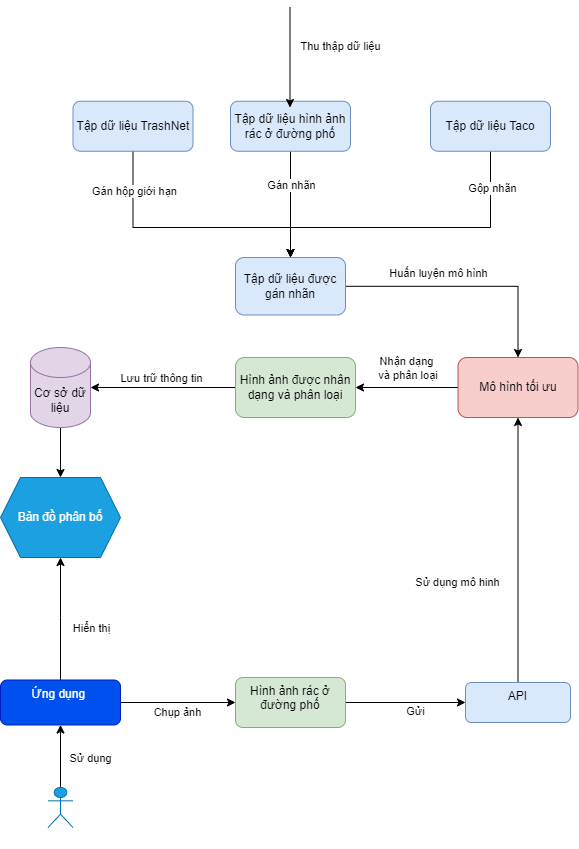
\includegraphics[width=0.8\textwidth]{sodo.png}
	\caption{Sơ đồ hệ thống}
	\label{fig:sodo}
\end{figure}

\end{document}


